\documentclass[preview]{standalone}
\usepackage{tkz-graph}
\begin{document}

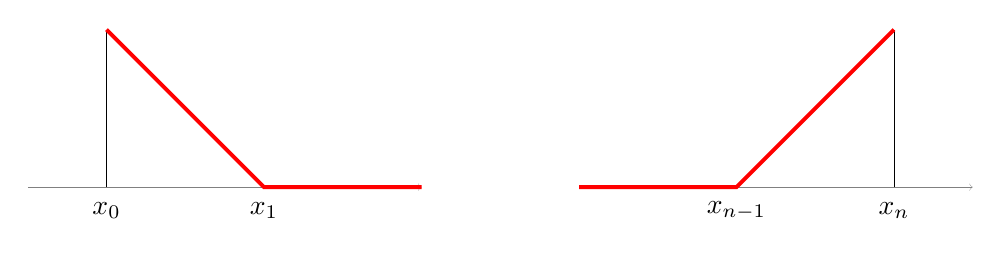
\begin{tikzpicture}
\draw[->,ultra  thin,color=gray] (1,0) -- (6, 0);
\draw[line width=0.1mm, color=black] (2,0) -- (2, 2);
\draw[line width=0.5mm, color=red] (2,2) -- (4,0) -- (6,0);
\draw (2, -0.3) node {$x_{0}$};
\draw (4, -0.3) node {$x_{1}$};
\draw[->,ultra  thin,color=gray] (8,0) -- (13, 0);
\draw[line width=0.1mm, color=black] (12,0) -- (12, 2);
\draw[line width=0.5mm, color=red] (8,0) -- (10,0) -- (12,2);
\draw (10, -0.3) node {$x_{n-1}$};
\draw (12, -0.3) node {$x_{n}$};
\end{tikzpicture}

\end{document}



После: convert pdf to png
https://convertio.co/pdf-png/



 






